
%% Beginning of file 'sample63.tex'
%%
%% Modified 2019 June
%%
%% This is a sample manuscript marked up using the
%% AASTeX v6.3 LaTeX 2e macros.
%%
%% AASTeX is now based on Alexey Vikhlinin's emulateapj.cls 
%% (Copyright 2000-2015).  See the classfile for details.

%% AASTeX requires revtex4-1.cls (http://publish.aps.org/revtex4/) and
%% other external packages (latexsym, graphicx, amssymb, longtable, and epsf).
%% All of these external packages should already be present in the modern TeX 
%% distributions.  If not they can also be obtained at www.ctan.org.

%% The first piece of markup in an AASTeX v6.x document is the \documentclass
%% command. LaTeX will ignore any data that comes before this command. The 
%% documentclass can take an optional argument to modify the output style.
%% The command below calls the preprint style which will produce a tightly 
%% typeset, one-column, single-spaced document.  It is the default and thus
%% does not need to be explicitly stated.
%%
%%
%% using aastex version 6.3
\documentclass{aastex63}

%% The default is a single spaced, 10 point font, single spaced article.
%% There are 5 other style options available via an optional argument. They
%% can be invoked like this:
%%
%% \documentclass[arguments]{aastex63}
%% 
%% where the layout options are:
%%
%%  twocolumn   : two text columns, 10 point font, single spaced article.
%%                This is the most compact and represent the final published
%%                derived PDF copy of the accepted manuscript from the publisher
%%  manuscript  : one text column, 12 point font, double spaced article.
%%  preprint    : one text column, 12 point font, single spaced article.  
%%  preprint2   : two text columns, 12 point font, single spaced article.
%%  modern      : a stylish, single text column, 12 point font, article with
%% 		  wider left and right margins. This uses the Daniel
%% 		  Foreman-Mackey and David Hogg design.
%%  RNAAS       : Preferred style for Research Notes which are by design 
%%                lacking an abstract and brief. DO NOT use \begin{abstract}
%%                and \end{abstract} with this style.
%%
%% Note that you can submit to the AAS Journals in any of these 6 styles.
%%
%% There are other optional arguments one can invoke to allow other stylistic
%% actions. The available options are:
%%
%%   astrosymb    : Loads Astrosymb font and define \astrocommands. 
%%   tighten      : Makes baselineskip slightly smaller, only works with 
%%                  the twocolumn substyle.
%%   times        : uses times font instead of the default
%%   linenumbers  : turn on lineno package.
%%   trackchanges : required to see the revision mark up and print its output
%%   longauthor   : Do not use the more compressed footnote style (default) for 
%%                  the author/collaboration/affiliations. Instead print all
%%                  affiliation information after each name. Creates a much 
%%                  longer author list but may be desirable for short 
%%                  author papers.
%% twocolappendix : make 2 column appendix.
%%   anonymous    : Do not show the authors, affiliations and acknowledgments 
%%                  for dual anonymous review.
%%
%% these can be used in any combination, e.g.
%%
%% \documentclass[twocolumn,linenumbers,trackchanges]{aastex63}
%%
%% AASTeX v6.* now includes \hyperref support. While we have built in specific
%% defaults into the classfile you can manually override them with the
%% \hypersetup command. For example,
%%
%% \hypersetup{linkcolor=red,citecolor=green,filecolor=cyan,urlcolor=magenta}
%%
%% will change the color of the internal links to red, the links to the
%% bibliography to green, the file links to cyan, and the external links to
%% magenta. Additional information on \hyperref options can be found here:
%% https://www.tug.org/applications/hyperref/manual.html#x1-40003
%%
%% Note that in v6.3 "bookmarks" has been changed to "true" in hyperref
%% to improve the accessibility of the compiled pdf file.
%%
%% If you want to create your own macros, you can do so
%% using \newcommand. Your macros should appear before
%% the \begin{document} command.
%%
\newcommand{\vdag}{(v)^\dagger}
\newcommand\aastex{AAS\TeX}
\newcommand\latex{La\TeX}

%% Reintroduced the \received and \accepted commands from AASTeX v5.2
\received{\today}
\revised{\today}
\accepted{\today}
%% Command to document which AAS Journal the manuscript was submitted to.
%% Adds "Submitted to " the argument.
\submitjournal{ApJL}

%% For manuscript that include authors in collaborations, AASTeX v6.3
%% builds on the \collaboration command to allow greater freedom to 
%% keep the traditional author+affiliation information but only show
%% subsets. The \collaboration command now must appear AFTER the group
%% of authors in the collaboration and it takes TWO arguments. The last
%% is still the collaboration identifier. The text given in this
%% argument is what will be shown in the manuscript. The first argument
%% is the number of author above the \collaboration command to show with
%% the collaboration text. If there are authors that are not part of any
%% collaboration the \nocollaboration command is used. This command takes
%% one argument which is also the number of authors above to show. A
%% dashed line is shown to indicate no collaboration. This example manuscript
%% shows how these commands work to display specific set of authors 
%% on the front page.
%%
%% For manuscript without any need to use \collaboration the 
%% \AuthorCollaborationLimit command from v6.2 can still be used to 
%% show a subset of authors.
%
%\AuthorCollaborationLimit=2
%
%% will only show Schwarz & Muench on the front page of the manuscript
%% (assuming the \collaboration and \nocollaboration commands are
%% commented out).
%%
%% Note that all of the author will be shown in the published article.
%% This feature is meant to be used prior to acceptance to make the
%% front end of a long author article more manageable. Please do not use
%% this functionality for manuscripts with less than 20 authors. Conversely,
%% please do use this when the number of authors exceeds 40.
%%
%% Use \allauthors at the manuscript end to show the full author list.
%% This command should only be used with \AuthorCollaborationLimit is used.

%% The following command can be used to set the latex table counters.  It
%% is needed in this document because it uses a mix of latex tabular and
%% AASTeX deluxetables.  In general it should not be needed.
%\setcounter{table}{1}

%%%%%%%%%%%%%%%%%%%%%%%%%%%%%%%%%%%%%%%%%%%%%%%%%%%%%%%%%%%%%%%%%%%%%%%%%%%%%%%%
%%
%% The following section outlines numerous optional output that
%% can be displayed in the front matter or as running meta-data.
%%
%% If you wish, you may supply running head information, although
%% this information may be modified by the editorial offices.
\shorttitle{GD\,394 and TESS}
\shortauthors{Wilson et al. 2020}
%%
%% You can add a light gray and diagonal water-mark to the first page 
%% with this command:
%% \watermark{text}
%% where "text", e.g. DRAFT, is the text to appear.  If the text is 
%% long you can control the water-mark size with:
%% \setwatermarkfontsize{dimension}
%% where dimension is any recognized LaTeX dimension, e.g. pt, in, etc.
%%
%%%%%%%%%%%%%%%%%%%%%%%%%%%%%%%%%%%%%%%%%%%%%%%%%%%%%%%%%%%%%%%%%%%%%%%%%%%%%%%%
\graphicspath{{./}{figures/}}
%% This is the end of the preamble.  Indicate the beginning of the
%% manuscript itself with \begin{document}.

\begin{document}

%\title{I'm Not Dead Yet: Optical detection of the periodic variability at the white dwarf GD\,394 with the Transiting Exoplanet Survey Satellite}

\title{Optical detection of the 1.1-day variability at the white dwarf GD\,394 with \textit{TESS}}

%% LaTeX will automatically break titles if they run longer than
%% one line. However, you may use \\ to force a line break if
%% you desire. In v6.3 you can include a footnote in the title.%% you desire. In v6.3 you can include a footnote in the title.



%% A significant change from earlier AASTEX versions is in the structure for 
%% calling author and affiliations. The change was necessary to implement 
%% auto-indexing of affiliations which prior was a manual process that could 
%% easily be tedious in large author manuscripts.
%%
%% The \author command is the same as before except it now takes an optional
%% argument which is the 16 digit ORCID. The syntax is:
%% \author[xxxx-xxxx-xxxx-xxxx]{Author Name}
%%
%% This will hyperlink the author name to the author's ORCID page. Note that
%% during compilation, LaTeX will do some limited checking of the format of
%% the ID to make sure it is valid. If the "orcid-ID.png" image file is 
%% present or in the LaTeX pathway, the OrcID icon will appear next to
%% the authors name.
%%
%% Use \affiliation for affiliation information. The old \affil is now aliased
%% to \affiliation. AASTeX v6.3 will automatically index these in the header.
%% When a duplicate is found its index will be the same as its previous entry.
%%
%% Note that \altaffilmark and \altaffiltext have been removed and thus 
%% can not be used to document secondary affiliations. If they are used latex
%% will issue a specific error message and quit. Please use multiple 
%% \affiliation calls for to document more than one affiliation.
%%
%% The new \altaffiliation can be used to indicate some secondary information
%% such as fellowships. This command produces a non-numeric footnote that is
%% set away from the numeric \affiliation footnotes.  NOTE that if an
%% \altaffiliation command is used it must come BEFORE the \affiliation call,
%% right after the \author command, in order to place the footnotes in
%% the proper location.
%%
%% Use \email to set provide email addresses. Each \email will appear on its
%% own line so you can put multiple email address in one \email call. A new
%% \correspondingauthor command is available in V6.3 to identify the
%% corresponding author of the manuscript. It is the author's responsibility
%% to make sure this name is also in the author list.
%%
%% While authors can be grouped inside the same \author and \affiliation
%% commands it is better to have a single author for each. This allows for
%% one to exploit all the new benefits and should make book-keeping easier.
%%
%% If done correctly the peer review system will be able to
%% automatically put the author and affiliation information from the manuscript
%% and save the corresponding author the trouble of entering it by hand.
\correspondingauthor{David J. Wilson}
\email{djwilson394\@gmail.com}

\author[0000-0001-9667-9449]{David J. Wilson}
\affil{McDonald Observatory, University of Texas at Austin, Austin, TX 78712}

\author{J. J. Hermes}
\affil{Department of Astronomy, Boston University, 725 Commonwealth Ave., Boston, MA 02215, USA}

\author{Boris T. G{\"a}nsicke}
\affil{Department of Physics, University of Warwick, Coventry CV4 7AL,UK}



%% Note that the \and command from previous versions of AASTeX is now
%% depreciated in this version as it is no longer necessary. AASTeX 
%% automatically takes care of all commas and "and"s between authors names.

%% AASTeX 6.3 has the new \collaboration and \nocollaboration commands to
%% provide the collaboration status of a group of authors. These commands 
%% can be used either before or after the list of corresponding authors. The
%% argument for \collaboration is the collaboration identifier. Authors are
%% encouraged to surround collaboration identifiers with ()s. The 
%% \nocollaboration command takes no argument and exists to indicate that
%% the nearby authors are not part of surrounding collaborations.

%% Mark off the abstract in the ``abstract'' environment. 
\begin{abstract}
Recent discoveries have demonstrated that planetary systems routinely survive the post-main sequence evolution of their host stars, leaving the resulting white dwarf with a rich circumsteller environment. Among the most intriguing of such hosts is the hot white dwarf GD\,394, exhibiting a unique $1.150\pm0.003$\,d flux variation detected in \textit{Extreme Ultraviolet Explorer} (\textit{EUVE}) observations in the mid 1990s. The variation has eluded a satisfactory explanation, but hypotheses include channeled accretion producing a dark spot of metals, occultation by a gas cloud from an evaporating planet, or heating from a flux tube produced by an orbiting iron-cored planetesimal. 

We present observations obtained with the \textit{Transiting Exoplanet Survey Satellite} (\textit{TESS}) of GD\,394. The space-based optical photometry demonstrates a $0.12\pm0.01$\% flux variation with a period of $1.146\pm 0.001$\,d, consistent with the \textit{EUVE} period and the first re-detection of the flux variation outside of the extreme ultraviolet. We describe the analysis of the \textit{TESS} light curve and measurement of the optical variation, and discuss the implications of our results for the various physical explanations put forward for the variability of GD\,394.    
%abstract has to be <250 words for ApJL

\end{abstract}

%% Keywords should appear after the \end{abstract} command. 
%% See the online documentation for the full list of available subject
%% keywords and the rules for their use.
\keywords{}

%% From the front matter, we move on to the body of the paper.
%% Sections are demarcated by \section and \subsection, respectively.
%% Observe the use of the LaTeX \label
%% command after the \subsection to give a symbolic KEY to the
%% subsection for cross-referencing in a \ref command.
%% You can use LaTeX's \ref and \label commands to keep track of
%% cross-references to sections, equations, tables, and figures.
%% That way, if you change the order of any elements, LaTeX will
%% automatically renumber them.
%%
%% We recommend that authors also use the natbib \citep
%% and \citet commands to identify citations.  The citations are
%% tied to the reference list via symbolic KEYs. The KEY corresponds
%% to the KEY in the \bibitem in the reference list below. 

\section{Introduction} \label{sec:intro}
GD\,394 is a hot, metal-polluted white dwarf that has challenged interpretation since its initial identification by \citet{giclasetal67-1}. Indeed, both of the descriptions in the preceding sentence are unquantified: Estimates for the effective temperature vary from 33000--41000\,K \citep{lajoie+bergeron07-1, barstowetal96-1} and the measured metal abundances, accretion rates, and species depend on the wavelength band and ionisation levels observed \citep{wilsonetal19-1}. However, the most intriguing aspect of GD\,394 is the detection by \citet{christianetal99-1} and \citet{dupuisetal00-1} of a sustained 25\% modulation of the extreme ultraviolet (EUV 70--380\,\AA) flux with a period of 1.15\,d in observations made in 1992--1996 with multiple instruments onboard the {\em Extreme Ultraviolet Explorer} ({\em EUVE}) satellite. This large-amplitude EUV modulation is so far unique among white dwarfs, and was hypothesised to be due to opacity changes induced by a spot of accreting metals moving in to and out of view with the white dwarf rotation. 

The metal spot hypothesis made two observable predictions. First, the strength of the metal lines in the white dwarf spectrum should vary in phase with the EUV variation. Second, there should be an anti-phase flux variation at optical wavelengths due to flux redistribution. Follow-up observations  by \citet{wilsonetal19-1} ruled out the first of these predictions, finding no change in the strength of strong Si, Fe and Al absorption lines in eight \textit{Hubble Space Telescope} (\textit{HST}) far ultraviolet (FUV, 1160-1700\,\AA) spectra sampling the full (putative) white dwarf spin cycle. They also searched SuperWASP photometry for optical variability, ruling out $\gtrsim$\,1\% changes in flux. Instead of a spot model, \citet{wilsonetal19-1} favoured a circumstellar explanation such as a gas cloud generated by an evaporating but non-transiting planet, similar to the ice giant detected in an $\approx$8--10\,d orbit of WD J0914+1914 by \citet{gaensickeetal19-1}. \citet{veras+wolszczan19-1} alternatively suggested that an orbiting, iron-rich planetesimal core could induce a magnetic flux tube connecting it to the white dwarf in GD\,394, heating the photosphere at the base of the tube to produce a hot spot. 
 
Here, we present observations of GD\,394 obtained using the {\em Transiting Exoplanet Survey Satellite} \citep[\textit{TESS},][]{rickeretal14-1} demonstrating that GD\,394 is indeed varying in the optical with a period in agreement with that detected previously in the EUV, but with a much smaller amplitude. Section \ref{sec:obs} details our analysis of the \textit{TESS} light curve. Section \ref{sec:disc} discusses the implications of the optical re-detection for the physical explanation of the variation at GD\,394. 

\begin{figure}
    \centering
    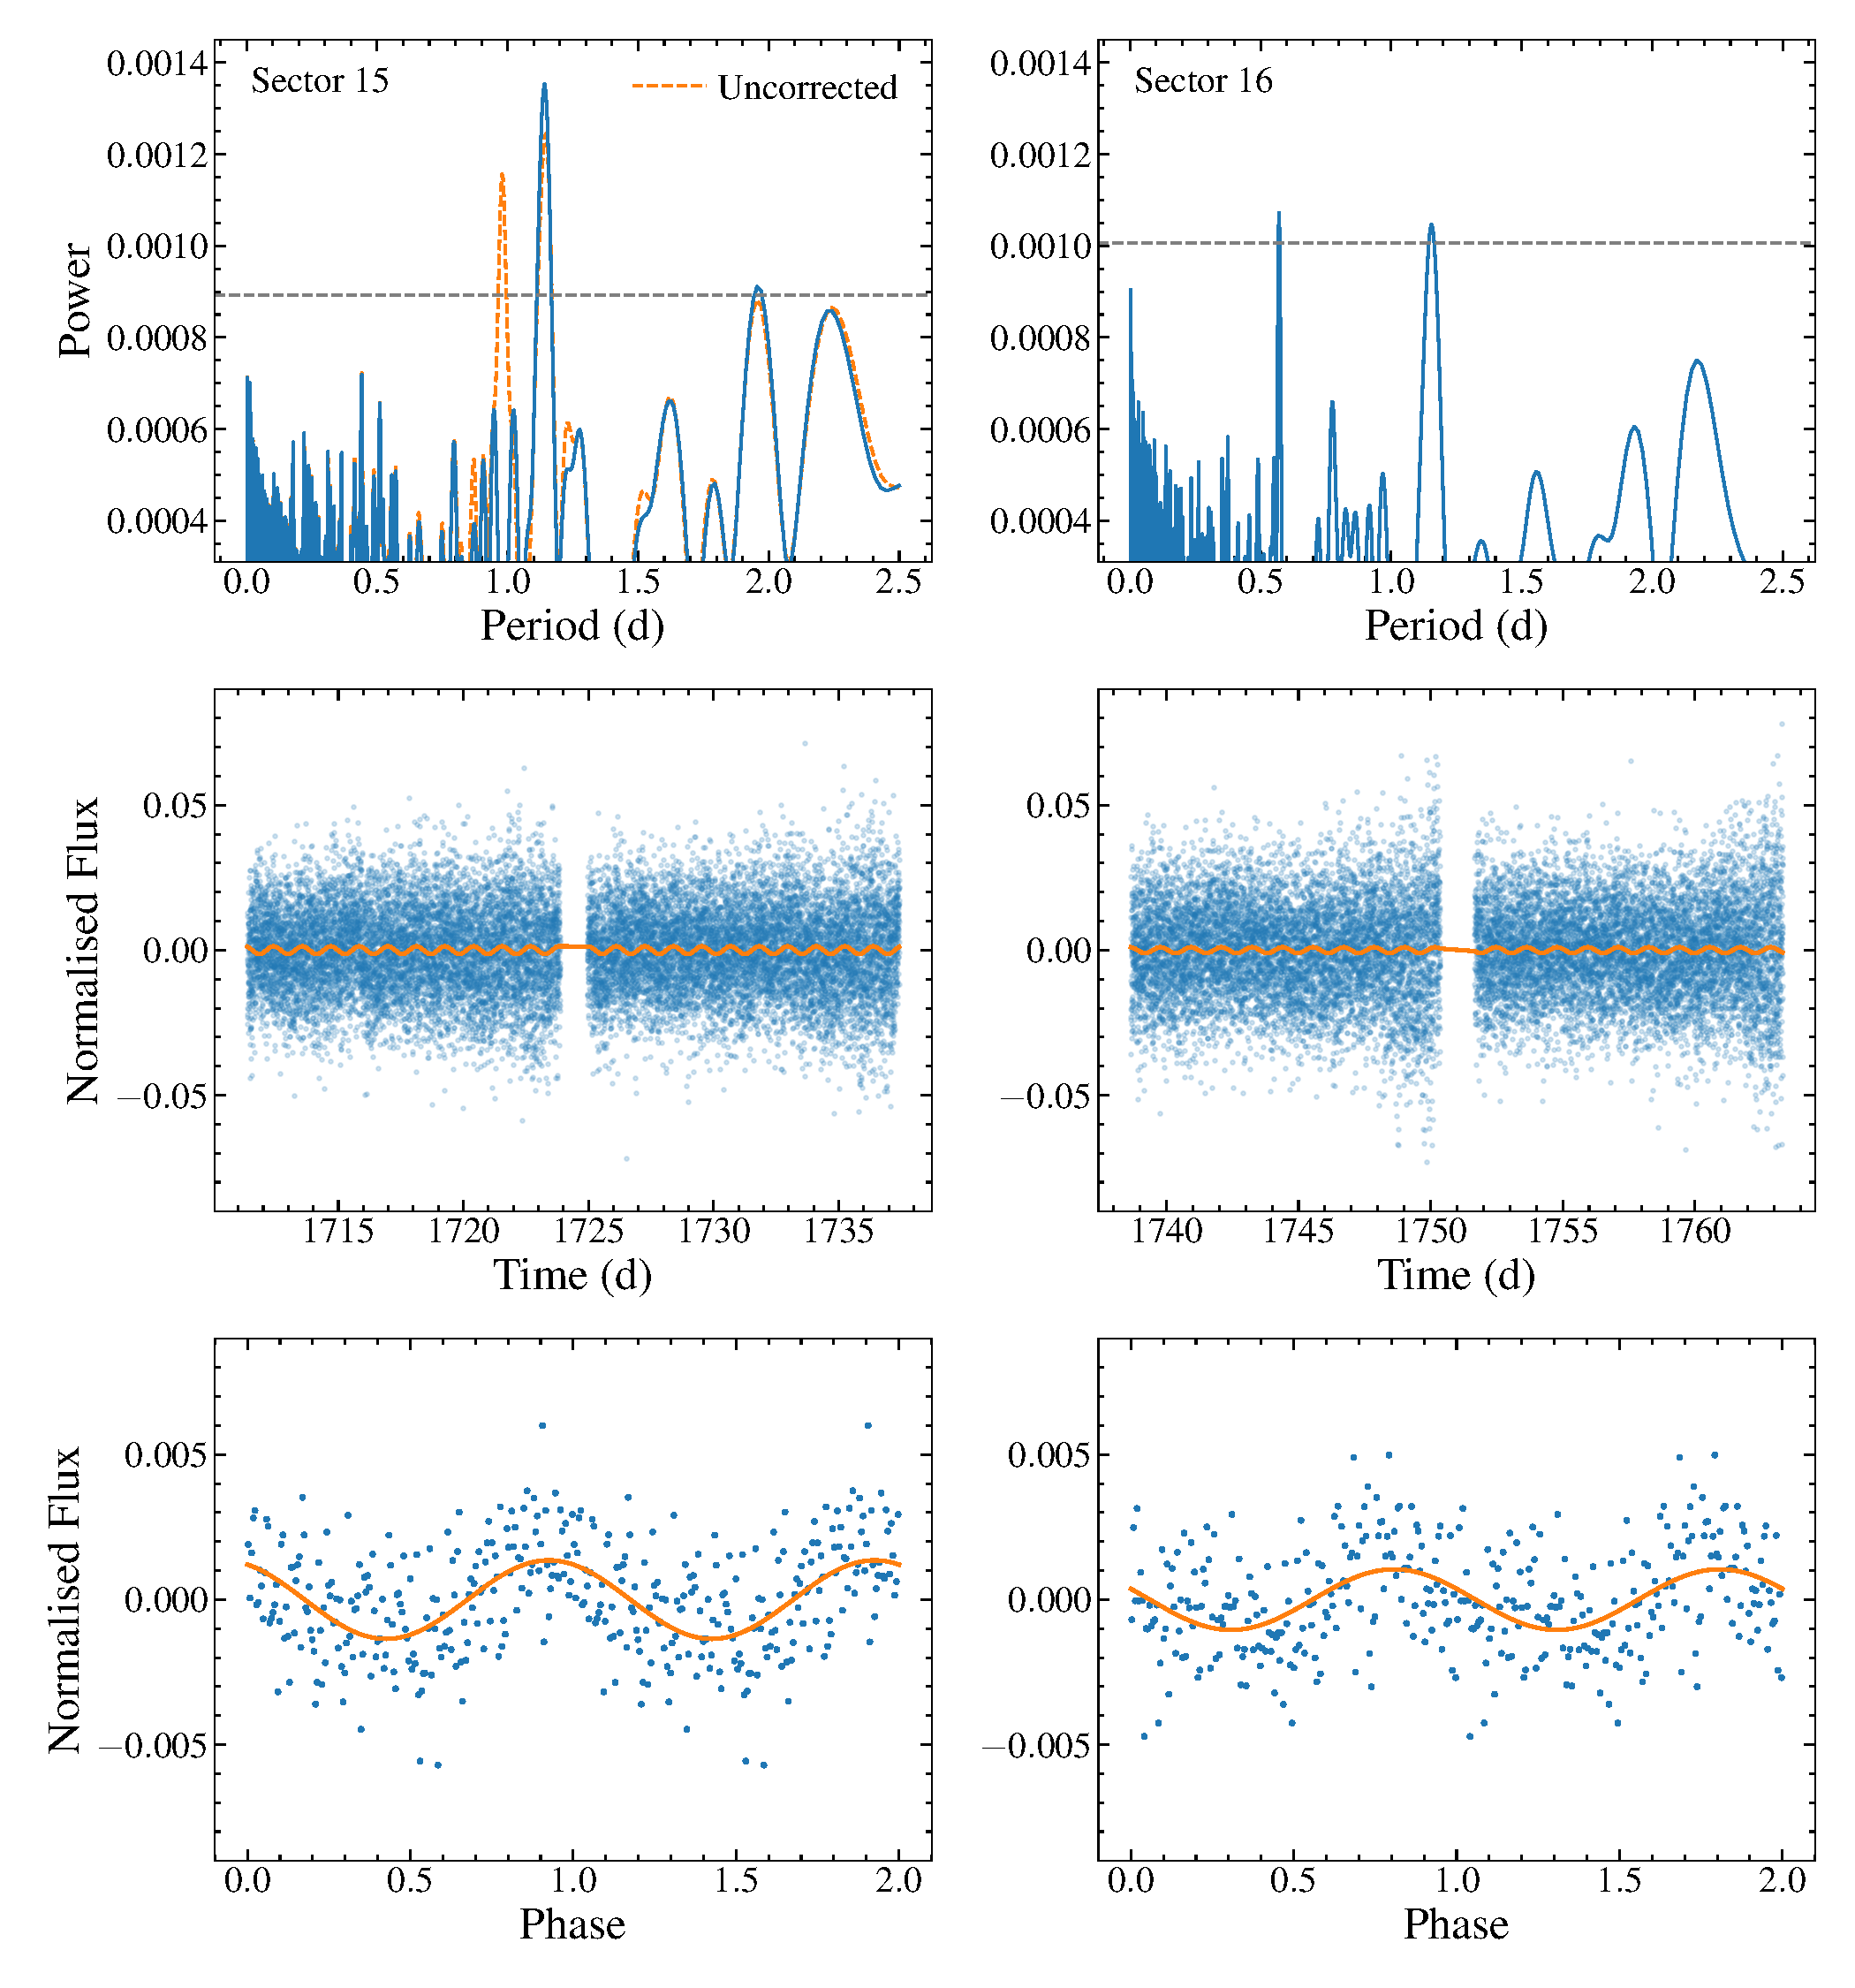
\includegraphics[width=\columnwidth]{gd394_tess_full.pdf}
    \caption{Top: Periodograms of the \textit{TESS} light curves of GD\,394 from Sectors 15 and 16. The grey dashed line shows the 99\% false alarm probability signal apparent in each sector, as discussed in the text. Significant signals at $1.1459\pm0.0033$\,d and $1.1547\pm0.0051$\,d  are detected in Sector 15 and 16 respectively. The $\approx 0.98$\,d signal apparent in Sector 15 is due to contamination from a nearby giant star. The first harmonic ($P$/2) of the 1.15\,d signal is detected in Sector 16. Middle: \textit{TESS} light curves of GD\,394 together with the sine fit used to measure the period and amplitude of the variation. The enhanced scatter at the end of each segment of the light curve is due to increased background Earthshine as the spacecraft approaches perigee. Bottom: Light curves folded onto the fitted period and binned to 40 steps. The cycle is repeated for clarity, and the model fit is overplotted in orange. }
    \label{fig:all_obs}
\end{figure}

% The median error bar for each sector is shown in the top-right.

%The orange dashed line shows the periodogram for Sector 15 before removal of the $\approx 0.98$\,d signal from a nearby star. 



%\begin{figure}
 %   \centering
  %  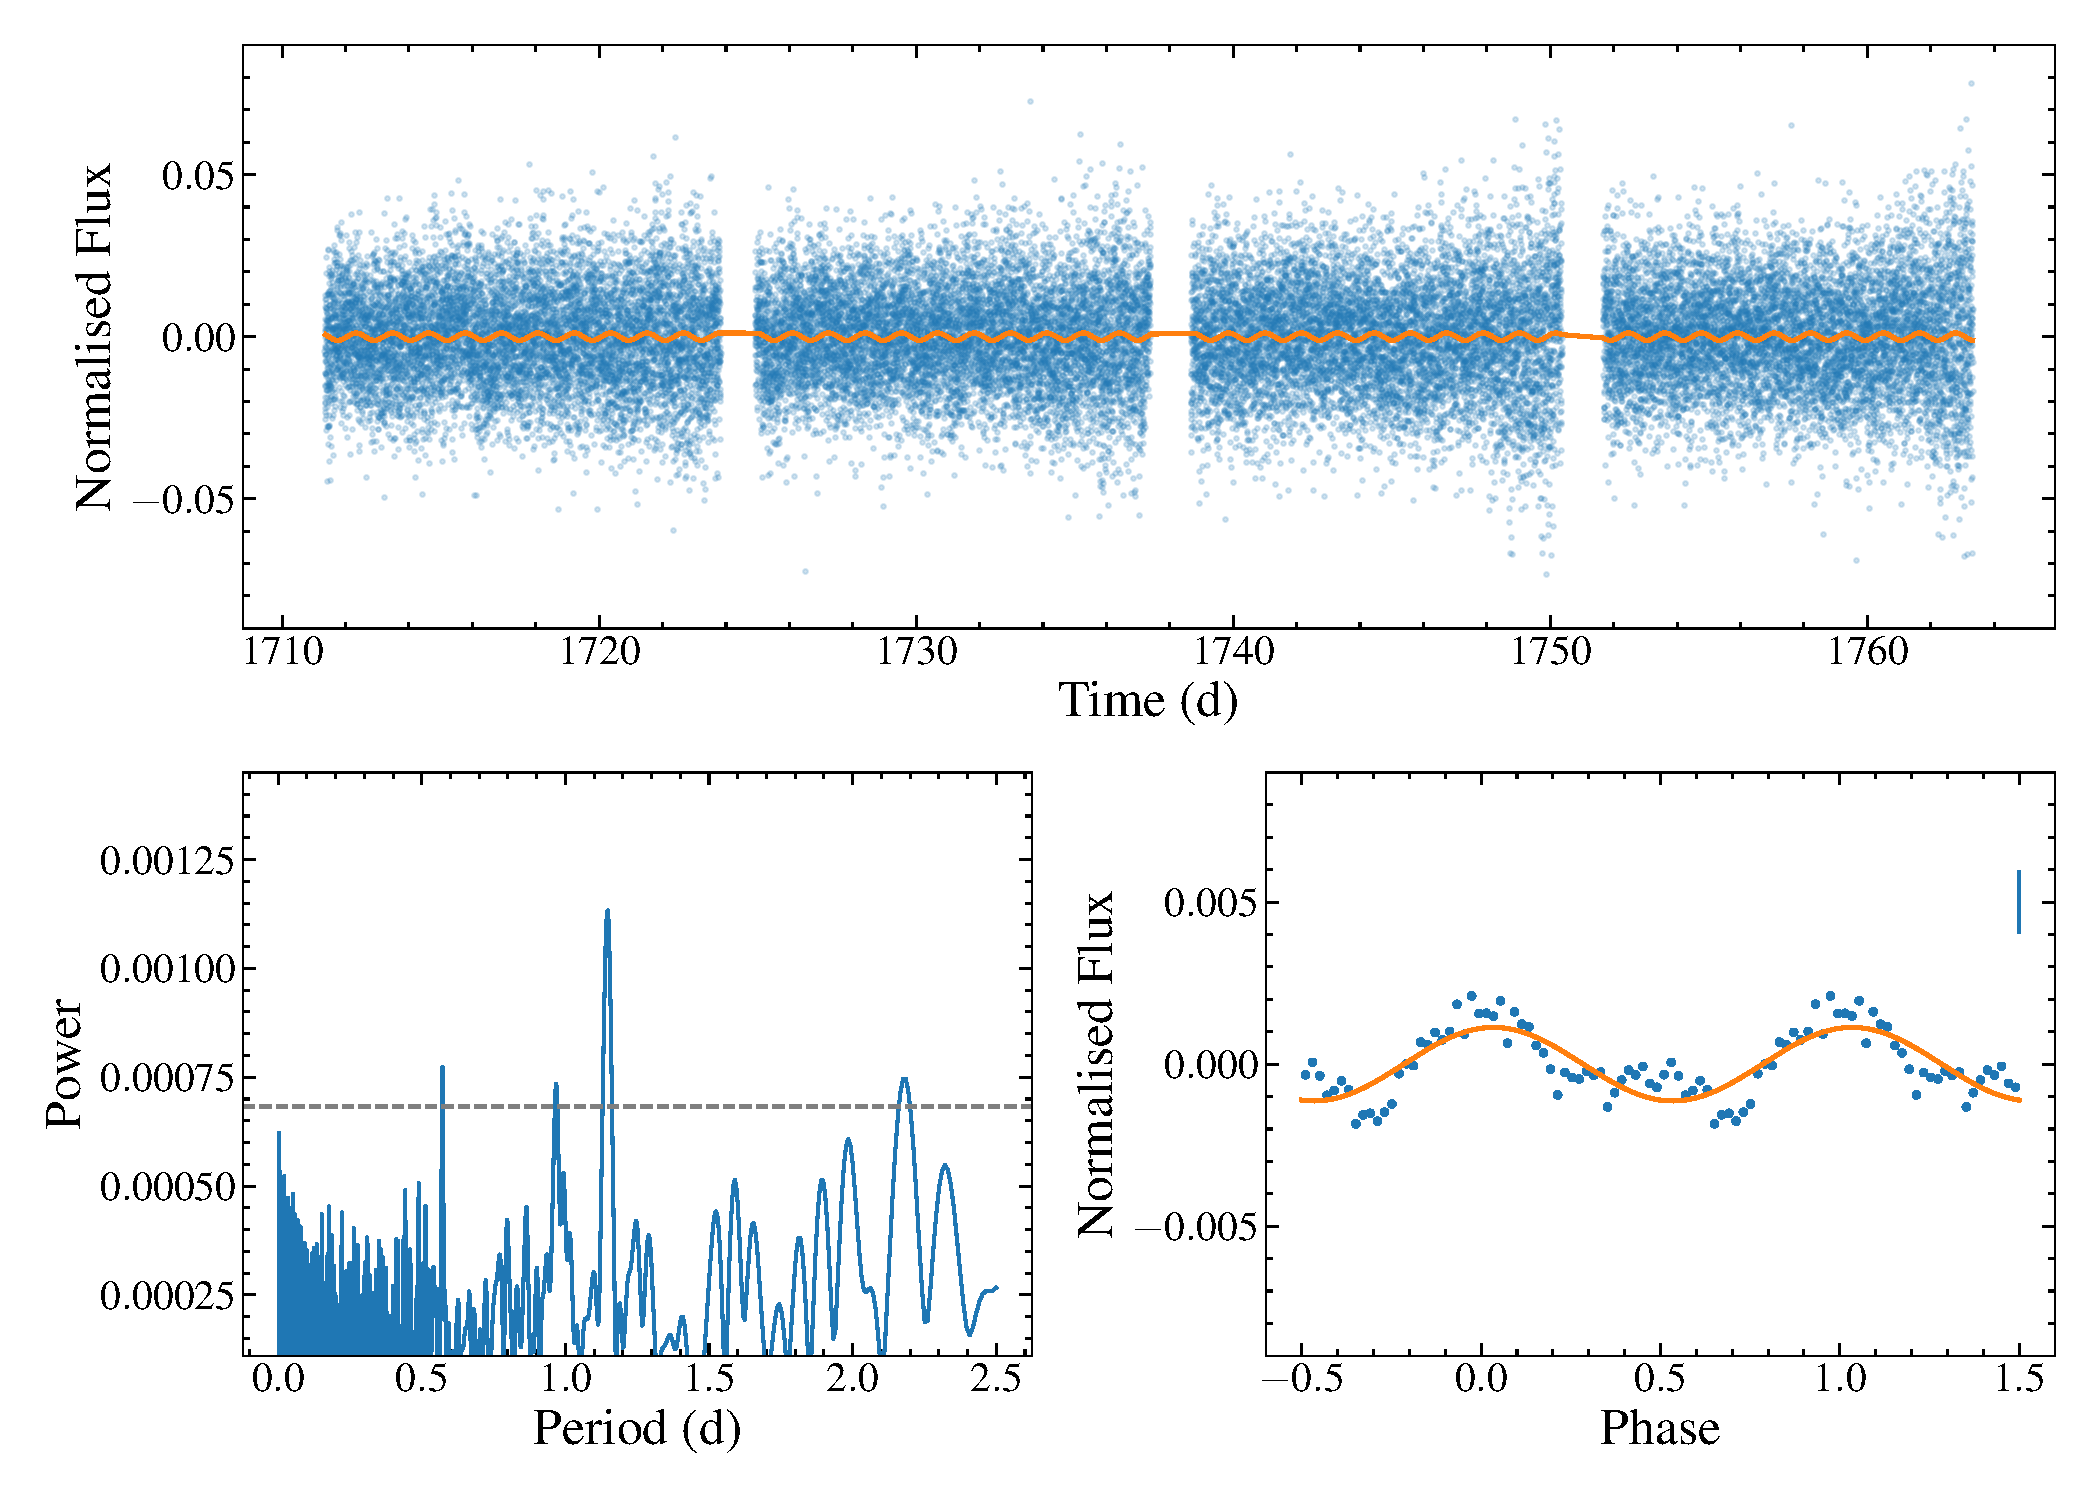
\includegraphics[width=\columnwidth]{gd394_tess_both.pdf}
   % \caption{Joint analysis of both Sectors, using the background-signal subtracted light curve for Sector 15. Top: The combined two-sector light curve (blue) with a fit to the variation in orange. Left: Periodogram of the combined light curve with the 99\% false alarm probability shown in grey. Right: Folded, binned light curve and model fit.}
   % \label{fig:both_obs}
%\end{figure}

\section{Observations} \label{sec:obs}

%textbf{NB ApJL limit is 5 figures.}

%\subsection{\textit{TESS}} \label{sec:tess} 
%\begin{figure}
 %   \centering
  %  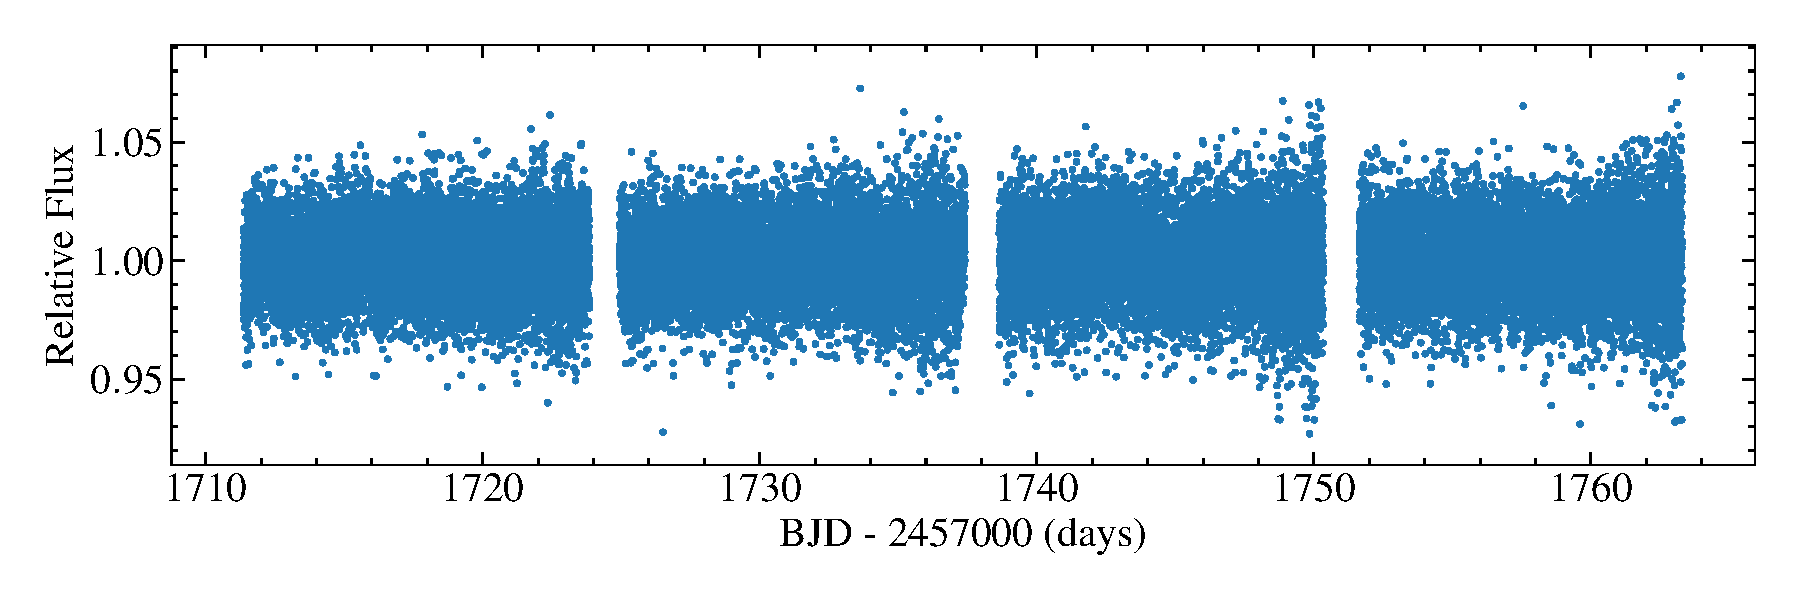
\includegraphics[width=\columnwidth]{gd394_tess_lc.pdf}
  %  \caption{Combined {\em TESS} light curve of GD\,394 with flagged points removed and normalised to a polynomial fit to each sector.}
  %  \label{fig:tess_lc}
%\end{figure}
GD\,394 (TIC 259773610, $T$=13.4\,mag) was observed by {\em TESS} in Camera~2 for 52 days in Sectors 15 and 16 (2019~August~15--2019~October~06), with three roughly one-day gaps at spacecraft perigee\footnote{See \textit{TESS} Data Release Notes at \url{http://archive.stsci.edu/tess/tess_drn.html}}. Data was returned with a two~minute cadence as requested in proposals G022077, G022028 and G022017, and processed using the Pre-Search  Data  Conditioning  Pipeline  \citep[PDC,][]{stumpeetal12-1} to remove common known instrumental trends.

\defcitealias{lightkurve18-1}{Lightkurve Collaboration, 2018}

We analysed the light curves from each sector separately. The light curves were retrieved from MAST\footnote{https://archive.stsci.edu/} and points marked with a quality flag were removed, as were any 5-sigma outliers above the median flux. The flux was normalised by subtracting a second-order polynomial fit. We generated Lomb-Scargle periodograms using the \texttt{Lightkurve} package \citepalias{lightkurve18-1} (Figure \ref{fig:all_obs}, top). A $\approx 1.15$\,d period is clearly detected in each sector, providing the first confirmation of the {\em EUVE} detection beyond the extreme ultraviolet. 

The Sector 15 periodogram contained a second peak at $\approx 0.98$\,d (orange dashed line in Figure \ref{fig:all_obs}). Using the \textit{TESS} pixel data, we found that this signal originates from a nearby giant star, TIC 259773551 (\textit{TESS} magnitude = 12.9). We have therefore ignored this periodicity; it only marginally adds to our  systematic uncertainties.

To ascertain the significance of the detected signals we calculated the false alarm probability (FAP) via the method described in \citet{hermesetal17-1,belletal19-1}. In short, we generated $10{,}000$ synthetic light curves for each sector, using the same time-axis but randomly shuffling the flux values. A periodogram was calculated for each synthetic light curve and the maximum amplitude recorded. We defined our 1\% FAP as the power below which the maximum amplitude in 99\% of our synthetic light curves fell (grey dashed line in Figure \ref{fig:all_obs}). As the signals in each light curve exceed this limit, we conclude that there is a less than one per\,cent probability that our detected signal is due to random chance in each sector, and therefore a $<$0.01\% chance of observing the same, random signal in both sectors. A $P/2$ harmonic of the expected signal is also detected with $< 1\%$ FAP in Sector 16. 


We then fit a sinusoid to each light curve using the peak measured from the periodogram as an initial guess for the period, shown in the middle panel of Figure \ref{fig:all_obs}.
The bottom panel shows the data folded onto the fitted period, clearly demonstrating the sinusoidal nature of the signal.

\begin{table}
    \centering
    \begin{tabular}{lccc}
        Sector & Mid-MJD (d) & Period (d) & Amplitude (\%)  \\ \hline
        \textit{EUVE} & $\approx50000$ & $1.15\pm0.003$ & $\approx25$ \\
         15 & 58724   &$1.1459\pm0.0033$ & $0.127\pm0.016$ \\
         16 & 58750 &$1.1547\pm0.0051$& $0.102\pm0.018$ \\
        % \textit{TESS} average & 58736 & $1.145\pm0.006$ & $0.21\pm0.04$ \\
        $15+16$ & 58736 & $1.1468\pm0.0014$ & $0.117\pm0.012$ \\
        Ephemeris (BJD):  & $2458737.560\pm0.018$ & \\
    \end{tabular}
    \caption{Measured periods and amplitudes for the variation at GD\,394. \textit{EUVE} measurements from \citet{dupuisetal00-1} are given as approximations as observations were obtained at multiple epochs with different instruments.} 
    \label{tab:peramp}
\end{table}

The periods and amplitudes for each sector are consistent to within 3$\sigma$, so we do not formally detect any amplitude or phase variability between the two sectors. However, the shape of the power spectrum is notably different between the two sectors. In particular, the amplitude of the $1.1547\pm0.0051$\,d signal in Sector 16 is weaker than the $1.1459\pm0.0033$ signal in Sector 15, and the $P/2$ harmonic is clearly detected in Sector 16 but not Sector 15.  

We combined the light curves from both sectors and repeated the analysis, finding a period of $1.1466\pm0.0015$\,days and an amplitude $0.117\pm0.012$\% in the {\em TESS} bandpass, centered at a wavelength of roughly 786.5\,nm. The ephemeris is defined as the peak of the model fit closest to the mid-point of the \textit{TESS} observations, $T_{\mathrm{Ephemeris}} =2458737.560\pm0.018$\,(BJD). Table \ref{tab:peramp} summarises the various period and amplitude measurements for GD\,394 from \textit{TESS} and \textit{EUVE}. 


%Re-reading Dupius +00, they did a very thorough job on the EUVE data, I don't think there's much more we can add, and can probably take their period as given.}

%\section{Discussion and Conclusion} \label{sec:disc}


\begin{figure}
    \centering
    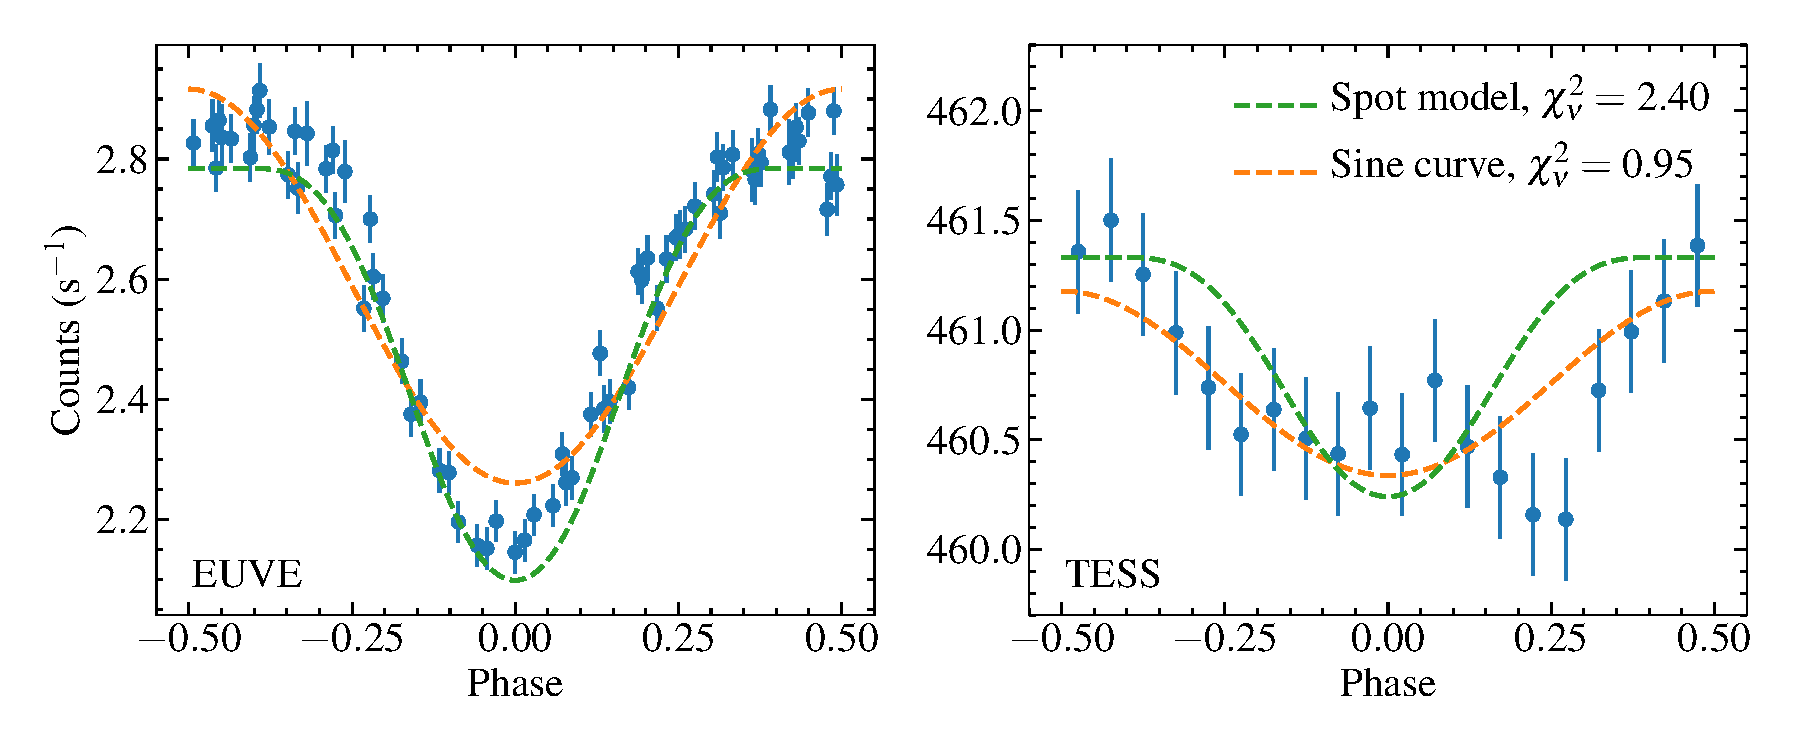
\includegraphics[width=\columnwidth]{euve_v_tess_mod_sin.pdf}
    \caption{Comparison of the \textit{EUVE} and \textit{TESS} signals. Left: Recreation of Fig. 6 of \citet{dupuisetal00-1} showing the \textit{EUVE} DS light curve. Right: 2-sector \textit{TESS} light curve folded onto the measured 1.1468\,d period and binned to 20 points. In both panels the dashed green and orange lines show model fits to each light curve using the \citet{dupuisetal00-1} spot model and a sinusoidal respectively.}
    \label{fig:euve}
\end{figure}

%The dashed line shows a model with the \textit{EUVE} best-fit parameters but with the opacity ratio reduced to 1\,\%.

\section{Discussion} \label{sec:disc}

The  $P = 1.145\pm 0.006$\,d periodic variation of GD\,394 in the {\em TESS} light curve is consistent with the $ 1.150\pm0.003$\,d period measured in the {\em EUVE} data by \citet{dupuisetal00-1}, with no strong evidence for period evolution in the roughly 24 years between the observations. On the other hand, the optical amplitude of $0.117\pm0.012$\% is much smaller than the $\approx$25\% variation in the EUV, and below the $\approx$1\,\% upper limits placed on FUV variation by \citet{wilsonetal19-1}.

Figure \ref{fig:euve} compares the folded \textit{EUVE} light curve and best-fit spot model from \citet{dupuisetal00-1} with the folded \textit{TESS} light curve. \citet{dupuisetal00-1} adopted a model where the spot is completely dark, with the ratio of the flux of the spot to the photosphere $kw =0$. To investigate whether the same spot is causing the \textit{TESS} variation, we fit a model keeping the geometry of the best-fit EUV model but varying the opacity. We find an $\approx$1\,\% flux ratio (i.e. $kw\approx0.99$ in the \citet{dupuisetal00-1} notation) provides a reasonable match to the folded \textit{TESS} light curveHowever, the sinusoidal model used to measure the period is statistically a better fit to the \textit{TESS} data despite being a poor model for the \textit{EUVE} light curve. The poor signal-to-noise ratio of the \textit{TESS} data dominates the fit, so confidently distinguishing between different models, and confirming whether the optical variation definitely has the same origin as the EUV variation, is not possible.

%As discussed below there is good reason to assume that they are linked, but we cannot rule out that the optical and EUV detection represent two separate events and/or variation mechanisms.          of the optical 1.15d modulation

%with further precision precluded by the low signal-to-noise ratio of the data. 

%Not sure how to phrase this, or even if it needs to be said

%However, equally good fits can be obtained by varying other parameters of the spot model, e.g. the angular size of the spot, so the \textit{TESS} data does not strongly support either way that the optical variation is caused by a spot with the same geometry as fitted to the \textit{EUVE} observations

%The \textit{TESS} data therefore neither strongly confirms nor rules out that the optical variation is caused by a spot with the same geometry as fitted to the \textit{EUVE} observations.  

Optical variation was a prediction of the metal spot model favoured by \citet{dupuisetal00-1} as an explanation for the EUV variation. However, the metal spot model was not supported by the non-detection of changes in FUV metal absorption line strengths by \citet{wilsonetal19-1}. It is possible that the spot has a variable opacity, appearing strongly at the time of the 1993--1996 \textit{EUVE} observations, fading by the time of the 2015 \textit{HST} observations but returning in time to be observed with 2019 \textit{TESS} observations (with the period fixed by the white dwarf rotation period). However, this is likely too strong an appeal to coincidence, especially considering that Si absorption line strengths in the 2015 \textit{HST} spectra were consistent with the strengths of the same lines detected in \textit{HST} spectra obtained in 1992 by \citet{shipmanetal95-2}. Figure \ref{fig:euve} shows that a lower opacity version of the spot model fitted to the \textit{EUVE} data does does not exactly describe the \textit{TESS} light curve, raising the possibility that the geometry of the spot may have changed. If the \textit{TESS} mission is extended long enough for GD\,394 to be reobserved then tests for changes in the variation amplitude and shape will be possible. 

We are left requiring a mechanism that will generate flux variations of 25\% in the EUV, 0.117\% in the optical, and $\lesssim 1$\% in the FUV (the upper limit placed by light curves extracted from the time-tagged \textit{HST} spectroscopy by \citet{wilsonetal19-1}. The suggestion by \citet{veras+wolszczan19-1} that the variation is due to a hot spot at the base of a magnetic flux tube may fit these criteria, as a sufficiently hot spot could provide the required amplitude in the EUV, with the flux quickly dropping away in the Rayleigh–Jeans tail to the low levels observed at longer wavelengths. However, this would require spot temperatures of $\gtrsim 10^5$\,K, and thus far no  magnetic field has been detected in high-resolution spectroscopy of GD\,394 \citep[$B_e \leq 12$\,kG,][]{dupuisetal00-1, wilsonetal19-1}. The generation of a flux tube requires an orbiting metal-rich planetary fragment which may be radio-loud, and thus radio observations might provide an opportunity to test this model.% \citep{veras+wolszczan19-1}. 
 
%Hmm...this is consistent with the EUV variation having higher amplitude at shorter wavelengths. Would show up nicely in the Chandra obs as well...}

The various explanations for the flux variations at GD\,394, including metal spots, occultation by an outflow from an orbiting planet, or a magnetically induced hot spot,  could be tested by searching for phase differences between the two wavebands: Out of phase variation would favour a metal spot; in phase variation would point to a circumstellar cause or a hot spot. In practice, phasing up the {\em EUVE} and {\em TESS} observations is impossible given cycle-count ambiguities in the decades-long gap between them. Therefore, new, contemporaneous EUV and high-precision optical observations are required, although this will be challenging given the currently available observing facilities.

The \textit{TESS} detection strengthens the connection between GD\,394 and WD\,J1855+4207 suggested by \citet{hallakounetal18-1}, both stars having high ($> 30000$\,K) effective temperatures, high ionisation-level metal absorption lines with strengths well above those predicted by their effective temperatures, and weak, many-hour period optical modulation \citep{maozetal15-1}. Proposed future missions such as \textit{ESCAPE} \citep{franceetal19-1} could search for EUV variation at WD\,J1855+4207, confirming whether or not it is truly a GD\,394 analogue.

%  to provide a larger test sample for the proposed physical explanations of the variation

In conclusion, the \textit{TESS} observations of GD\,394 reveal the same 1.15\,d periodicity at optical wavelengths that was initially identified in the EUV more than two decades ago. The very small amplitude of the optical modulation, 0.12\,\%, explains why this signal remained undetected in previous ground-based observations of GD\,394. A physical explanation for the modulation now detected in two wavebands remains elusive.

\acknowledgments
We thank A. Vanderburg for useful advice regarding contamination from nearby stars in \textit{TESS}, and J. Dupuis for sharing the \textit{EUVE} light curves. JJH acknowledges support by the National Aeronautics and Space Administration through the \textit{TESS} Guest Investigator Program (80NSSC19K0378). This paper includes data collected by the \textit{TESS} mission. Funding for the \textit{TESS} mission is provided by the NASA Explorer Program.

%% To help institutions obtain information on the effectiveness of their 
%% telescopes the AAS Journals has created a group of keywords for telescope 
%% facilities.
%
%% Following the acknowledgments section, use the following syntax and the
%% \facility{} or \facilities{} macros to list the keywords of facilities used 
%% in the research for the paper.  Each keyword is check against the master 
%% list during copy editing.  Individual instruments can be provided in 
%% parentheses, after the keyword, but they are not verified.

\vspace{5mm}
\facilities{\textit{TESS} }

%% Similar to \facility{}, there is the optional \software command to allow 
%% authors a place to specify which programs were used during the creation of 
%% the manusscript. Authors should list each code and include either a
%% citation or url to the code inside ()s when available.
\defcitealias{astropy18-1}{Astropy Collaboration, 2018}

\software{Astropy \citepalias{astropy18-1}, Lightkurve \citepalias{lightkurve18-1}}

%% Appendix material should be preceded with a single \appendix command.
%% There should be a \section command for each appendix. Mark appendix
%% subsections with the same markup you use in the main body of the paper.

%% Each Appendix (indicated with \section) will be lettered A, B, C, etc.
%% The equation counter will reset when it encounters the \appendix
%% command and will number appendix equations (A1), (A2), etc. The
%% Figure and Table counter will not reset.




%\appendix

%\section{Appendix information}

\bibliographystyle{aasjournal}
\bibliography{aabib}

%% This command is needed to show the entire author+affiliation list when
%% the collaboration and author truncation commands are used.  It has to
%% go at the end of the manuscript.
%\allauthors

%% Include this line if you are using the \added, \replaced, \deleted
%% commands to see a summary list of all changes at the end of the article.
%\listofchanges

\end{document}
